%%%%%%%%%%%%%%%%%%%%%%%%%%%%%%%%%%%%%%%%%%%%%%%%%%%%%%%%%%%%%%%%%%%%%%
% This layout was adapted from one found at latextemplates.com which
% was adapted from another.
%
% License: CC BY-NC-SA 3.0
% (http://creativecommons.org/licenses/by-nc-sa/3.0/)
%
% Original header:
%
% This is a LaTeX version of the sample laboratory report from
% Virginia Tech's copyrighted 08-09 CHEM 1045/1046 lab manual.
% Reproduction of this one appendix section for academic purposes
% should fall under fair use.
%
%%%%%%%%%%%%%%%%%%%%%%%%%%%%%%%%%%%%%%%%%%%%%%%%%%%%%%%%%%%%%%%%%%%%%%

\documentclass{article}

\usepackage{graphicx} % Lets us use images
%\usepackage[acronym]{glossaries} % Lets us use acronyms
\usepackage{siunitx} % SI units in math mode

\author{}
\title{ELEC-313 \\ Lab 1: Amplifier Models \\ }
\date{\today}

% This loads the acronym definitions and creates a glossary.
% \makeglossaries is required (I think), even though we don't print
% out a separate glossary page.  The first time an acronym is used,
% LaTeX writes the whole word (defining the acronym), and after that
% it prints only the acronym.  There is an example of their use in the
% caption of the table in the Results section.
%\loadglsentries{acronyms} % Actually loads 'acronyms.tex'
%\makeglossaries

\begin{document}

\maketitle % Inserts title, author, and date from above

 \begin{center}
   \begin{tabular}{lr}
    Date Performed: & September 11, 2013 \\
    Partners: & Charles Pittman \\
              & Stephen W-something? \\
  \end{tabular}
\end{center}

\pagebreak

% Removes indentation from paragraphs: \setlength\parindent{0pt}

% Number the enumerate environment (unordered lists) by letter:
\renewcommand{\labelenumi}{\alph{enumi}.}

% And now we start our actual text.  Note that each chunk is
% designated by the \section{} tag.
\section{Objective}

% \label{} is used when you want to refer to something later.  It's
% simply an identifier for whatever container it's in.  See
% Conclusions section for an example of \ref{}.
\label{sec:objective}

The objective is to verify the equivalence of four circuits used to model an amplifier, shown in Figure~\ref{fig:amp_models}.

\section{Schematics}
\label{sec:schematics}

% The asterisk after section inhibits the numbering of the section.
\subsection*{Circuit Tested}
\label{sec:ckt_tested}

% Insert a picture:
\begin{figure}[h]
  \label{fig:circuit}
  \centering
  % File is at "./img/circuit.png".  Plain LaTeX only supports .eps
  % files.  Other LaTeX compilers support different formats.  I use
  % pdflatex.
    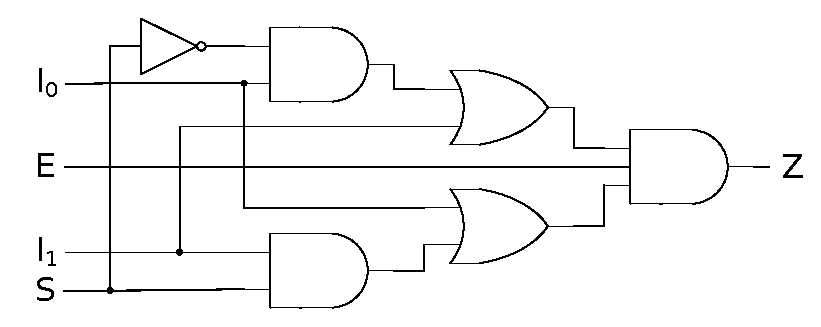
\includegraphics[]{img/circuit}
  \caption{Circuit being tested.  $C_1 = C_2 = \SI{1}{\micro\farad}$}
\end{figure}

\subsection*{Test Configuration}
\label{sec:test_config}

\begin{figure}[h]
  \centering
  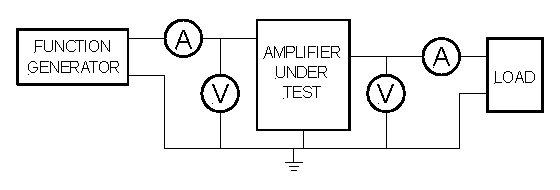
\includegraphics[]{img/test_config}
  \caption{Test Configuration}
  \label{fig:test_config}
\end{figure}

\section{Procedure}
\label{sec:procedure}

Lorem ipsum dolor sit amet, consectetuer adipiscing elit. Donec
hendrerit tempor tellus. Donec pretium posuere tellus. Proin quam
nisl, tincidunt et, mattis eget, convallis nec, purus. Cum sociis
natoque penatibus et magnis dis parturient montes, nascetur ridiculus
mus. Nulla posuere. Donec vitae dolor. Nullam tristique diam non
turpis. Cras placerat accumsan nulla. Nullam rutrum. Nam vestibulum
accumsan nisl.

\section{Results}

% We use the table environment just to hold the caption and label.
% I've never tried putting them inside the tabular environment yet,
% but it may work:
\begin{table}[h]
  \label{tab:table_01}
  \centering
  \begin{tabular}{*{4}{c}}
    \textbf{Name} & \textbf{Nominal} & \textbf{Measured} & \textbf{\% Error} \\
    & ($\si{\kilo\ohm}$) & ($\si{\kilo\ohm}$) & \\
    \hline
    $R_1$ & 1 & 0.986 & 1.40 \\
    $R_2$ & 10 & 9.88 & 1.20 \\
    $R_3$ & 1 & 0.983 & 1.70 \\
  \end{tabular}
  \caption{Comparison of labelled and actual resistance.}
\end{table}

\begin{table}[h]
  \label{tab:table_02}
  \centering
  \begin{tabular}{*{7}{c}}
    & \multicolumn{2}{c}{\textbf{Voltage}} & \multicolumn{2}{c}{\textbf{Current}} & \multicolumn{2}{c}{\textbf{Gain}} \\
    & $V_i$ & $V_o$ & $I_i$ & $I_o$ & $A_v$ & $A_i$ \\
    & $(\si{\milli\volt_{rms}})$ & $(\si{\volt_{rms}})$ & $(\si{\milli\ampere_{rms}})$ & $(\si{\milli\ampere_{rms}})$ & & \\
    \hline
    \textbf{No Load} & 200 & 1.98 & 0.2 & nil & 9.9 & nil \\
    \textbf{Load} & 200 & 1.98 & 0.2 & 9.52 & 9.9 & 47.6 \\
  \end{tabular}
  \caption{Comparison of electrical characteristics of the amplifier under load.}
\end{table}

\section{Conclusions}
\label{sec:conclusion}

In Table~\ref{tab:table_01}, lorem ipsum dolor sit amet, consectetuer
adipiscing elit. Donec hendrerit tempor tellus. Donec pretium posuere
tellus. Proin quam nisl, tincidunt et, mattis eget, convallis nec,
purus. Cum sociis natoque penatibus et magnis dis parturient montes,
nascetur ridiculus mus. Nulla posuere. Donec vitae dolor. Nullam
tristique diam non turpis. Cras placerat accumsan nulla. Nullam
rutrum. Nam vestibulum accumsan nisl.

Nullam eu ante vel est convallis dignissim. Fusce suscipit, wisi nec
facilisis facilisis, est dui fermentum leo, quis tempor ligula erat
quis odio. Nunc porta vulputate tellus. Nunc rutrum turpis sed
pede. Sed bibendum. Aliquam posuere. Nunc aliquet, augue nec
adipiscing interdum, lacus tellus malesuada massa, quis varius mi
purus non odio. Pellentesque condimentum, magna ut suscipit hendrerit,
ipsum augue ornare nulla, non luctus diam neque sit amet
urna. Curabitur vulputate vestibulum lorem. Fusce sagittis, libero non
molestie mollis, magna orci ultrices dolor, at vulputate neque nulla
lacinia eros. Sed id ligula quis est convallis tempor. Curabitur
lacinia pulvinar nibh. Nam a sapien.

\section*{Equations}

% \[ and \] designate "math mode" (just like $ did).  Note, this is
% also how we get special characters and pretty-print equations.
\[\%_{error} = \frac{|measured - nominal|}{nominal} \times 100\%\]
\[R_o = \frac{V_{noload} - V_{load}}{I_{load}}\]
\[R_i = \frac{V_i}{I_i}\]
\[A_v = \frac{V_o}{V_i}\]
\[A_i = A_v \left(\frac{R_i}{R_o}\right)\]
\[G_m = \frac{A_v}{R_o}\]
\[R_m = A_v R_i\]

\section{Appendix}
\label{sec:appendix}

\begin{figure}[h]
  \centering
  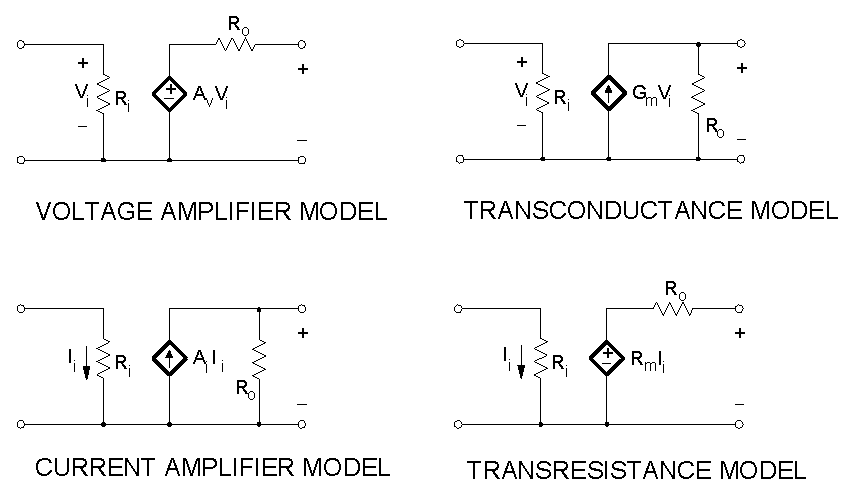
\includegraphics[]{img/amp_models}
  \caption{Four equivalent models of an amplifier}
  \label{fig:amp_models}
\end{figure}
\end{document}
